\documentclass[1p]{elsarticle_modified}
%\bibliographystyle{elsarticle-num}

%\usepackage[colorlinks]{hyperref}
%\usepackage{abbrmath_seonhwa} %\Abb, \Ascr, \Acal ,\Abf, \Afrak
\usepackage{amsfonts}
\usepackage{amssymb}
\usepackage{amsmath}
\usepackage{amsthm}
\usepackage{scalefnt}
\usepackage{amsbsy}
\usepackage{kotex}
\usepackage{caption}
\usepackage{subfig}
\usepackage{color}
\usepackage{graphicx}
\usepackage{xcolor} %% white, black, red, green, blue, cyan, magenta, yellow
\usepackage{float}
\usepackage{setspace}
\usepackage{hyperref}

\usepackage{tikz}
\usetikzlibrary{arrows}

\usepackage{multirow}
\usepackage{array} % fixed length table
\usepackage{hhline}

%%%%%%%%%%%%%%%%%%%%%
\makeatletter
\renewcommand*\env@matrix[1][\arraystretch]{%
	\edef\arraystretch{#1}%
	\hskip -\arraycolsep
	\let\@ifnextchar\new@ifnextchar
	\array{*\c@MaxMatrixCols c}}
\makeatother %https://tex.stackexchange.com/questions/14071/how-can-i-increase-the-line-spacing-in-a-matrix
%%%%%%%%%%%%%%%

\usepackage[normalem]{ulem}

\newcommand{\msout}[1]{\ifmmode\text{\sout{\ensuremath{#1}}}\else\sout{#1}\fi}
%SOURCE: \msout is \stkout macro in https://tex.stackexchange.com/questions/20609/strikeout-in-math-mode

\newcommand{\cancel}[1]{
	\ifmmode
	{\color{red}\msout{#1}}
	\else
	{\color{red}\sout{#1}}
	\fi
}

\newcommand{\add}[1]{
	{\color{blue}\uwave{#1}}
}

\newcommand{\replace}[2]{
	\ifmmode
	{\color{red}\msout{#1}}{\color{blue}\uwave{#2}}
	\else
	{\color{red}\sout{#1}}{\color{blue}\uwave{#2}}
	\fi
}

\newcommand{\Sol}{\mathcal{S}} %segment
\newcommand{\D}{D} %diagram
\newcommand{\A}{\mathcal{A}} %arc


%%%%%%%%%%%%%%%%%%%%%%%%%%%%%5 test

\def\sl{\operatorname{\textup{SL}}(2,\Cbb)}
\def\psl{\operatorname{\textup{PSL}}(2,\Cbb)}
\def\quan{\mkern 1mu \triangleright \mkern 1mu}

\theoremstyle{definition}
\newtheorem{thm}{Theorem}[section]
\newtheorem{prop}[thm]{Proposition}
\newtheorem{lem}[thm]{Lemma}
\newtheorem{ques}[thm]{Question}
\newtheorem{cor}[thm]{Corollary}
\newtheorem{defn}[thm]{Definition}
\newtheorem{exam}[thm]{Example}
\newtheorem{rmk}[thm]{Remark}
\newtheorem{alg}[thm]{Algorithm}

\newcommand{\I}{\sqrt{-1}}
\begin{document}

%\begin{frontmatter}
%
%\title{Boundary parabolic representations of knots up to 8 crossings}
%
%%% Group authors per affiliation:
%\author{Yunhi Cho} 
%\address{Department of Mathematics, University of Seoul, Seoul, Korea}
%\ead{yhcho@uos.ac.kr}
%
%
%\author{Seonhwa Kim} %\fnref{s_kim}}
%\address{Center for Geometry and Physics, Institute for Basic Science, Pohang, 37673, Korea}
%\ead{ryeona17@ibs.re.kr}
%
%\author{Hyuk Kim}
%\address{Department of Mathematical Sciences, Seoul National University, Seoul 08826, Korea}
%\ead{hyukkim@snu.ac.kr}
%
%\author{Seokbeom Yoon}
%\address{Department of Mathematical Sciences, Seoul National University, Seoul, 08826,  Korea}
%\ead{sbyoon15@snu.ac.kr}
%
%\begin{abstract}
%We find all boundary parabolic representation of knots up to 8 crossings.
%
%\end{abstract}
%\begin{keyword}
%    \MSC[2010] 57M25 
%\end{keyword}
%
%\end{frontmatter}

%\linenumbers
%\tableofcontents
%
\newcommand\colored[1]{\textcolor{white}{\rule[-0.35ex]{0.8em}{1.4ex}}\kern-0.8em\color{red} #1}%
%\newcommand\colored[1]{\textcolor{white}{ #1}\kern-2.17ex	\textcolor{white}{ #1}\kern-1.81ex	\textcolor{white}{ #1}\kern-2.15ex\color{red}#1	}

{\Large $\underline{12n_{0423}~(K12n_{0423})}$}

\setlength{\tabcolsep}{10pt}
\renewcommand{\arraystretch}{1.6}
\vspace{1cm}\begin{tabular}{m{100pt}>{\centering\arraybackslash}m{274pt}}
\multirow{5}{120pt}{
	\centering
	\includegraphics[width=112pt]{../../../GIT/diagram.site/Diagrams/png/2512_12n_0423.png}\\
\ \ \ A knot diagram\footnotemark}&
\allowdisplaybreaks
\textbf{Linearized knot diagam} \\
\cline{2-2}
 &
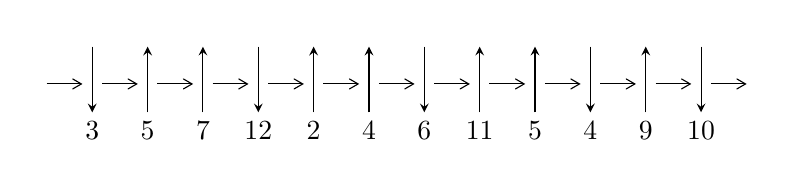
\begin{tikzpicture}[x=20pt, y=17pt]
	% nodes
	\node (C0) at (0, 0) {};
	\node (C1) at (1, 0) {};
	\node (C1U) at (1, +1) {};
	\node (C1D) at (1, -1) {3};

	\node (C2) at (2, 0) {};
	\node (C2U) at (2, +1) {};
	\node (C2D) at (2, -1) {5};

	\node (C3) at (3, 0) {};
	\node (C3U) at (3, +1) {};
	\node (C3D) at (3, -1) {7};

	\node (C4) at (4, 0) {};
	\node (C4U) at (4, +1) {};
	\node (C4D) at (4, -1) {12};

	\node (C5) at (5, 0) {};
	\node (C5U) at (5, +1) {};
	\node (C5D) at (5, -1) {2};

	\node (C6) at (6, 0) {};
	\node (C6U) at (6, +1) {};
	\node (C6D) at (6, -1) {4};

	\node (C7) at (7, 0) {};
	\node (C7U) at (7, +1) {};
	\node (C7D) at (7, -1) {6};

	\node (C8) at (8, 0) {};
	\node (C8U) at (8, +1) {};
	\node (C8D) at (8, -1) {11};

	\node (C9) at (9, 0) {};
	\node (C9U) at (9, +1) {};
	\node (C9D) at (9, -1) {5};

	\node (C10) at (10, 0) {};
	\node (C10U) at (10, +1) {};
	\node (C10D) at (10, -1) {4};

	\node (C11) at (11, 0) {};
	\node (C11U) at (11, +1) {};
	\node (C11D) at (11, -1) {9};

	\node (C12) at (12, 0) {};
	\node (C12U) at (12, +1) {};
	\node (C12D) at (12, -1) {10};
	\node (C13) at (13, 0) {};

	% arrows
	\draw[->,>={angle 60}]
	(C0) edge (C1) (C1) edge (C2) (C2) edge (C3) (C3) edge (C4) (C4) edge (C5) (C5) edge (C6) (C6) edge (C7) (C7) edge (C8) (C8) edge (C9) (C9) edge (C10) (C10) edge (C11) (C11) edge (C12) (C12) edge (C13) ;	\draw[->,>=stealth]
	(C1U) edge (C1D) (C2D) edge (C2U) (C3D) edge (C3U) (C4U) edge (C4D) (C5D) edge (C5U) (C6D) edge (C6U) (C7U) edge (C7D) (C8D) edge (C8U) (C9D) edge (C9U) (C10U) edge (C10D) (C11D) edge (C11U) (C12U) edge (C12D) ;
	\end{tikzpicture} \\
\hhline{~~} \\& 
\textbf{Solving Sequence} \\ \cline{2-2} 
 &
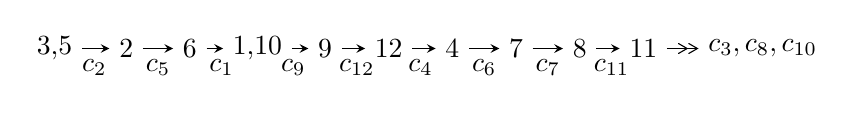
\begin{tikzpicture}[x=23pt, y=7pt]
	% node
	\node (A0) at (-1/8, 0) {3,5};
	\node (A1) at (1, 0) {2};
	\node (A2) at (2, 0) {6};
	\node (A3) at (49/16, 0) {1,10};
	\node (A4) at (33/8, 0) {9};
	\node (A5) at (41/8, 0) {12};
	\node (A6) at (49/8, 0) {4};
	\node (A7) at (57/8, 0) {7};
	\node (A8) at (65/8, 0) {8};
	\node (A9) at (73/8, 0) {11};
	\node (C1) at (1/2, -1) {$c_{2}$};
	\node (C2) at (3/2, -1) {$c_{5}$};
	\node (C3) at (5/2, -1) {$c_{1}$};
	\node (C4) at (29/8, -1) {$c_{9}$};
	\node (C5) at (37/8, -1) {$c_{12}$};
	\node (C6) at (45/8, -1) {$c_{4}$};
	\node (C7) at (53/8, -1) {$c_{6}$};
	\node (C8) at (61/8, -1) {$c_{7}$};
	\node (C9) at (69/8, -1) {$c_{11}$};
	\node (A10) at (11, 0) {$c_{3},c_{8},c_{10}$};

	% edge
	\draw[->,>=stealth]	
	(A0) edge (A1) (A1) edge (A2) (A2) edge (A3) (A3) edge (A4) (A4) edge (A5) (A5) edge (A6) (A6) edge (A7) (A7) edge (A8) (A8) edge (A9) ;
	\draw[->>,>={angle 60}]	
	(A9) edge (A10);
\end{tikzpicture} \\ 

\end{tabular} \\

\footnotetext{
The image of knot diagram is generated by the software ``\textbf{Draw programme}" developed by Andrew Bartholomew(\url{http://www.layer8.co.uk/maths/draw/index.htm\#Running-draw}), where we modified some parts for our purpose(\url{https://github.com/CATsTAILs/LinksPainter}).
}\phantom \\ \newline 
\centering \textbf{Ideals for irreducible components\footnotemark of $X_{\text{par}}$} 
 
\begin{align*}
I^u_{1}&=\langle 
1231339 u^{16}-5163151 u^{15}+\cdots+19124224 b-5476095,\\
\phantom{I^u_{1}}&\phantom{= \langle  }-9673313 u^{16}+16707789 u^{15}+\cdots+9562112 a-54216803,\;u^{17}-2 u^{16}+\cdots+5 u+1\rangle \\
I^u_{2}&=\langle 
-3 u^3+u^2+4 b-2 u-1,\;- u^3+u^2+2 a-2 u+1,\;u^4+u^2+u+1\rangle \\
I^u_{3}&=\langle 
a^4+a^3 u+2 a^2+a u+b+u+2,\;a^5- a^4+2 a^3- a^2+a-1,\;u^2+1\rangle \\
I^u_{4}&=\langle 
-2048 u^9+33496 u^8+\cdots+334809 b+864245,\\
\phantom{I^u_{4}}&\phantom{= \langle  }535181 u^9-69173 u^8+\cdots+5691753 a-2597382,\\
\phantom{I^u_{4}}&\phantom{= \langle  }u^{10}- u^8+15 u^6- u^5+57 u^4+7 u^3+56 u^2+12 u+17\rangle \\
I^u_{5}&=\langle 
u^5+u^3- u^2+b,\;u^5+2 u^3- u^2+a+u-1,\;u^6- u^5+2 u^4-2 u^3+2 u^2-2 u+1\rangle \\
\\
\end{align*}
\raggedright * 5 irreducible components of $\dim_{\mathbb{C}}=0$, with total 47 representations.\\
\footnotetext{All coefficients of polynomials are rational numbers. But the coefficients are sometimes approximated in decimal forms when there is not enough margin.}
\newpage
\renewcommand{\arraystretch}{1}
\centering \section*{I. $I^u_{1}= \langle 1.23\times10^{6} u^{16}-5.16\times10^{6} u^{15}+\cdots+1.91\times10^{7} b-5.48\times10^{6},\;-9.67\times10^{6} u^{16}+1.67\times10^{7} u^{15}+\cdots+9.56\times10^{6} a-5.42\times10^{7},\;u^{17}-2 u^{16}+\cdots+5 u+1 \rangle$}
\flushleft \textbf{(i) Arc colorings}\\
\begin{tabular}{m{7pt} m{180pt} m{7pt} m{180pt} }
\flushright $a_{3}=$&$\begin{pmatrix}1\\0\end{pmatrix}$ \\
\flushright $a_{5}=$&$\begin{pmatrix}0\\u\end{pmatrix}$ \\
\flushright $a_{2}=$&$\begin{pmatrix}1\\u^2\end{pmatrix}$ \\
\flushright $a_{6}=$&$\begin{pmatrix}u\\u^3+u\end{pmatrix}$ \\
\flushright $a_{1}=$&$\begin{pmatrix}u^2+1\\u^2\end{pmatrix}$ \\
\flushright $a_{10}=$&$\begin{pmatrix}1.01163 u^{16}-1.74729 u^{15}+\cdots+11.6261 u+5.66996\\-0.0643864 u^{16}+0.269980 u^{15}+\cdots-1.56569 u+0.286343\end{pmatrix}$ \\
\flushright $a_{9}=$&$\begin{pmatrix}1.01163 u^{16}-1.74729 u^{15}+\cdots+11.6261 u+5.66996\\-0.299164 u^{16}+0.733070 u^{15}+\cdots-3.95716 u+0.0103754\end{pmatrix}$ \\
\flushright $a_{12}=$&$\begin{pmatrix}0.521430 u^{16}-1.40337 u^{15}+\cdots+2.34977 u-1.07163\\0.297738 u^{16}-0.653196 u^{15}+\cdots+2.42019 u+0.284846\end{pmatrix}$ \\
\flushright $a_{4}=$&$\begin{pmatrix}0.0312500 u^{15}-0.0625000 u^{14}+\cdots+0.156250 u+1.03125\\- u^2\end{pmatrix}$ \\
\flushright $a_{7}=$&$\begin{pmatrix}0.0312500 u^{16}-0.0625000 u^{15}+\cdots+0.156250 u^{2}+2.03125 u\\u\end{pmatrix}$ \\
\flushright $a_{8}=$&$\begin{pmatrix}0.0312500 u^{16}-0.0625000 u^{15}+\cdots+0.156250 u^{2}+2.03125 u\\u^5+u^3+u\end{pmatrix}$ \\
\flushright $a_{11}=$&$\begin{pmatrix}0.874375 u^{16}-1.76166 u^{15}+\cdots+11.3348 u+4.82131\\-0.142742 u^{16}+0.397649 u^{15}+\cdots-2.44474 u+0.0854782\end{pmatrix}$\\&\end{tabular}
\flushleft \textbf{(ii) Obstruction class $= -1$}\\~\\
\flushleft \textbf{(iii) Cusp Shapes $= -\frac{45218375}{76496896} u^{16}+\frac{24809901}{10928128} u^{15}+\cdots+\frac{290991179}{38248448} u+\frac{522539755}{76496896}$}\\~\\
\newpage\renewcommand{\arraystretch}{1}
\flushleft \textbf{(iv) u-Polynomials at the component}\newline \\
\begin{tabular}{m{50pt}|m{274pt}}
Crossings & \hspace{64pt}u-Polynomials at each crossing \\
\hline $$\begin{aligned}c_{1},c_{7}\end{aligned}$$&$\begin{aligned}
&u^{17}+8 u^{15}+\cdots-15 u-1
\end{aligned}$\\
\hline $$\begin{aligned}c_{2},c_{3},c_{5}\\c_{6}\end{aligned}$$&$\begin{aligned}
&u^{17}+2 u^{16}+\cdots+5 u-1
\end{aligned}$\\
\hline $$\begin{aligned}c_{4}\end{aligned}$$&$\begin{aligned}
&u^{17}+6 u^{16}+\cdots+12 u+4
\end{aligned}$\\
\hline $$\begin{aligned}c_{8},c_{11}\end{aligned}$$&$\begin{aligned}
&u^{17}+5 u^{16}+\cdots-97 u-16
\end{aligned}$\\
\hline $$\begin{aligned}c_{9}\end{aligned}$$&$\begin{aligned}
&2(2 u^{17}-5 u^{16}+\cdots+16 u+568)
\end{aligned}$\\
\hline $$\begin{aligned}c_{10}\end{aligned}$$&$\begin{aligned}
&2(2 u^{17}-7 u^{16}+\cdots-6391 u+13778)
\end{aligned}$\\
\hline $$\begin{aligned}c_{12}\end{aligned}$$&$\begin{aligned}
&u^{17}-3 u^{16}+\cdots-800 u+256
\end{aligned}$\\
\hline
\end{tabular}\\~\\
\newpage\renewcommand{\arraystretch}{1}
\flushleft \textbf{(v) Riley Polynomials at the component}\newline \\
\begin{tabular}{m{50pt}|m{274pt}}
Crossings & \hspace{64pt}Riley Polynomials at each crossing \\
\hline $$\begin{aligned}c_{1},c_{7}\end{aligned}$$&$\begin{aligned}
&y^{17}+16 y^{16}+\cdots-243 y-1
\end{aligned}$\\
\hline $$\begin{aligned}c_{2},c_{3},c_{5}\\c_{6}\end{aligned}$$&$\begin{aligned}
&y^{17}+8 y^{15}+\cdots-15 y-1
\end{aligned}$\\
\hline $$\begin{aligned}c_{4}\end{aligned}$$&$\begin{aligned}
&y^{17}+2 y^{16}+\cdots-104 y-16
\end{aligned}$\\
\hline $$\begin{aligned}c_{8},c_{11}\end{aligned}$$&$\begin{aligned}
&y^{17}-25 y^{16}+\cdots-2207 y-256
\end{aligned}$\\
\hline $$\begin{aligned}c_{9}\end{aligned}$$&$\begin{aligned}
&4(4 y^{17}-145 y^{16}+\cdots-145152 y-322624)
\end{aligned}$\\
\hline $$\begin{aligned}c_{10}\end{aligned}$$&$\begin{aligned}
&4(4 y^{17}-109 y^{16}+\cdots-6.94790\times10^{8} y-1.89833\times10^{8})
\end{aligned}$\\
\hline $$\begin{aligned}c_{12}\end{aligned}$$&$\begin{aligned}
&y^{17}+39 y^{16}+\cdots+316416 y-65536
\end{aligned}$\\
\hline
\end{tabular}\\~\\
\newpage\flushleft \textbf{(vi) Complex Volumes and Cusp Shapes}
$$\begin{array}{c|c|c}  
\text{Solutions to }I^u_{1}& \I (\text{vol} + \sqrt{-1}CS) & \text{Cusp shape}\\
 \hline 
\begin{aligned}
u &= -0.717924 + 0.486358 I \\
a &= \phantom{-}0.853936 - 0.745729 I \\
b &= \phantom{-}0.307111 - 0.292541 I\end{aligned}
 & \phantom{-}1.26458 - 1.13730 I & \phantom{-}3.35116 + 1.82167 I \\ \hline\begin{aligned}
u &= -0.717924 - 0.486358 I \\
a &= \phantom{-}0.853936 + 0.745729 I \\
b &= \phantom{-}0.307111 + 0.292541 I\end{aligned}
 & \phantom{-}1.26458 + 1.13730 I & \phantom{-}3.35116 - 1.82167 I \\ \hline\begin{aligned}
u &= -0.026424 + 0.757016 I \\
a &= \phantom{-}0.71710 + 1.42840 I \\
b &= \phantom{-}0.234197 + 0.550904 I\end{aligned}
 & \phantom{-}3.54267 - 4.48886 I & \phantom{-}11.22908 + 5.05916 I \\ \hline\begin{aligned}
u &= -0.026424 - 0.757016 I \\
a &= \phantom{-}0.71710 - 1.42840 I \\
b &= \phantom{-}0.234197 - 0.550904 I\end{aligned}
 & \phantom{-}3.54267 + 4.48886 I & \phantom{-}11.22908 - 5.05916 I \\ \hline\begin{aligned}
u &= \phantom{-}0.711308 + 1.176950 I \\
a &= -0.256063 - 0.466323 I \\
b &= -0.293782 + 0.033385 I\end{aligned}
 & -1.05610 + 6.71672 I & \phantom{-}0.12255 - 2.58272 I \\ \hline\begin{aligned}
u &= \phantom{-}0.711308 - 1.176950 I \\
a &= -0.256063 + 0.466323 I \\
b &= -0.293782 - 0.033385 I\end{aligned}
 & -1.05610 - 6.71672 I & \phantom{-}0.12255 + 2.58272 I \\ \hline\begin{aligned}
u &= -1.48564\phantom{ +0.000000I} \\
a &= -2.63464\phantom{ +0.000000I} \\
b &= -2.25227\phantom{ +0.000000I}\end{aligned}
 & \phantom{-}4.37099\phantom{ +0.000000I} & -1.92960\phantom{ +0.000000I} \\ \hline\begin{aligned}
u &= \phantom{-}0.051104 + 0.476773 I \\
a &= -0.70597 - 1.39720 I \\
b &= -0.525015 - 0.475256 I\end{aligned}
 & -0.95916 - 1.44555 I & -0.42899 + 2.81466 I \\ \hline\begin{aligned}
u &= \phantom{-}0.051104 - 0.476773 I \\
a &= -0.70597 + 1.39720 I \\
b &= -0.525015 + 0.475256 I\end{aligned}
 & -0.95916 + 1.44555 I & -0.42899 - 2.81466 I \\ \hline\begin{aligned}
u &= -0.185924 + 0.218364 I \\
a &= \phantom{-}4.27912 + 0.21207 I \\
b &= \phantom{-}0.454654 - 0.748287 I\end{aligned}
 & \phantom{-}1.91786 - 0.70287 I & \phantom{-}4.74657 - 1.86210 I\\
 \hline 
 \end{array}$$\newpage$$\begin{array}{c|c|c}  
\text{Solutions to }I^u_{1}& \I (\text{vol} + \sqrt{-1}CS) & \text{Cusp shape}\\
 \hline 
\begin{aligned}
u &= -0.185924 - 0.218364 I \\
a &= \phantom{-}4.27912 - 0.21207 I \\
b &= \phantom{-}0.454654 + 0.748287 I\end{aligned}
 & \phantom{-}1.91786 + 0.70287 I & \phantom{-}4.74657 + 1.86210 I \\ \hline\begin{aligned}
u &= \phantom{-}0.98623 + 1.52887 I \\
a &= -1.163130 + 0.777324 I \\
b &= -2.24771 - 0.01624 I\end{aligned}
 & \phantom{-}17.7964 + 14.2831 I & \phantom{-}2.56357 - 5.88484 I \\ \hline\begin{aligned}
u &= \phantom{-}0.98623 - 1.52887 I \\
a &= -1.163130 - 0.777324 I \\
b &= -2.24771 + 0.01624 I\end{aligned}
 & \phantom{-}17.7964 - 14.2831 I & \phantom{-}2.56357 + 5.88484 I \\ \hline\begin{aligned}
u &= -0.96033 + 1.57079 I \\
a &= \phantom{-}0.924952 + 0.534960 I \\
b &= \phantom{-}1.98481 + 0.05465 I\end{aligned}
 & \phantom{-}17.6776 - 6.3252 I & \phantom{-}2.67569 + 2.04454 I \\ \hline\begin{aligned}
u &= -0.96033 - 1.57079 I \\
a &= \phantom{-}0.924952 - 0.534960 I \\
b &= \phantom{-}1.98481 - 0.05465 I\end{aligned}
 & \phantom{-}17.6776 + 6.3252 I & \phantom{-}2.67569 - 2.04454 I \\ \hline\begin{aligned}
u &= \phantom{-}1.88478 + 0.57916 I \\
a &= \phantom{-}0.917377 - 0.559017 I \\
b &= \phantom{-}1.58688 + 0.23145 I\end{aligned}
 & \phantom{-}7.80121 + 3.61191 I & \phantom{-}6.17391 - 2.86781 I \\ \hline\begin{aligned}
u &= \phantom{-}1.88478 - 0.57916 I \\
a &= \phantom{-}0.917377 + 0.559017 I \\
b &= \phantom{-}1.58688 - 0.23145 I\end{aligned}
 & \phantom{-}7.80121 - 3.61191 I & \phantom{-}6.17391 + 2.86781 I\\
 \hline 
 \end{array}$$\newpage\newpage\renewcommand{\arraystretch}{1}
\centering \section*{II. $I^u_{2}= \langle -3 u^3+u^2+4 b-2 u-1,\;- u^3+u^2+2 a-2 u+1,\;u^4+u^2+u+1 \rangle$}
\flushleft \textbf{(i) Arc colorings}\\
\begin{tabular}{m{7pt} m{180pt} m{7pt} m{180pt} }
\flushright $a_{3}=$&$\begin{pmatrix}1\\0\end{pmatrix}$ \\
\flushright $a_{5}=$&$\begin{pmatrix}0\\u\end{pmatrix}$ \\
\flushright $a_{2}=$&$\begin{pmatrix}1\\u^2\end{pmatrix}$ \\
\flushright $a_{6}=$&$\begin{pmatrix}u\\u^3+u\end{pmatrix}$ \\
\flushright $a_{1}=$&$\begin{pmatrix}u^2+1\\u^2\end{pmatrix}$ \\
\flushright $a_{10}=$&$\begin{pmatrix}\frac{1}{2} u^3-\frac{1}{2} u^2+u-\frac{1}{2}\\\frac{3}{4} u^3-\frac{1}{4} u^2+\frac{1}{2} u+\frac{1}{4}\end{pmatrix}$ \\
\flushright $a_{9}=$&$\begin{pmatrix}\frac{1}{2} u^3-\frac{1}{2} u^2+u-\frac{1}{2}\\\frac{5}{4} u^3-\frac{3}{4} u^2+\frac{1}{2} u+\frac{3}{4}\end{pmatrix}$ \\
\flushright $a_{12}=$&$\begin{pmatrix}u^2+1\\u^2\end{pmatrix}$ \\
\flushright $a_{4}=$&$\begin{pmatrix}u^3- u^2\\- u^2\end{pmatrix}$ \\
\flushright $a_{7}=$&$\begin{pmatrix}- u^3- u^2-1\\u\end{pmatrix}$ \\
\flushright $a_{8}=$&$\begin{pmatrix}- u^2-1\\- u^2\end{pmatrix}$ \\
\flushright $a_{11}=$&$\begin{pmatrix}\frac{1}{2} u^3+\frac{1}{2} u^2+u+\frac{1}{2}\\\frac{5}{4} u^3+\frac{1}{4} u^2+\frac{1}{2} u+\frac{3}{4}\end{pmatrix}$\\&\end{tabular}
\flushleft \textbf{(ii) Obstruction class $= 1$}\\~\\
\flushleft \textbf{(iii) Cusp Shapes $= \frac{79}{16} u^3-\frac{85}{16} u^2-\frac{21}{8} u+\frac{93}{16}$}\\~\\
\newpage\renewcommand{\arraystretch}{1}
\flushleft \textbf{(iv) u-Polynomials at the component}\newline \\
\begin{tabular}{m{50pt}|m{274pt}}
Crossings & \hspace{64pt}u-Polynomials at each crossing \\
\hline $$\begin{aligned}c_{1}\end{aligned}$$&$\begin{aligned}
&u^4-2 u^3+3 u^2- u+1
\end{aligned}$\\
\hline $$\begin{aligned}c_{2},c_{3}\end{aligned}$$&$\begin{aligned}
&u^4+u^2+u+1
\end{aligned}$\\
\hline $$\begin{aligned}c_{4}\end{aligned}$$&$\begin{aligned}
&u^4-3 u^3+4 u^2-3 u+2
\end{aligned}$\\
\hline $$\begin{aligned}c_{5},c_{6}\end{aligned}$$&$\begin{aligned}
&u^4+u^2- u+1
\end{aligned}$\\
\hline $$\begin{aligned}c_{7}\end{aligned}$$&$\begin{aligned}
&u^4+2 u^3+3 u^2+u+1
\end{aligned}$\\
\hline $$\begin{aligned}c_{8}\end{aligned}$$&$\begin{aligned}
&(u+1)^4
\end{aligned}$\\
\hline $$\begin{aligned}c_{9},c_{10}\end{aligned}$$&$\begin{aligned}
&2(2 u^4+3 u^3+4 u^2+3 u+1)
\end{aligned}$\\
\hline $$\begin{aligned}c_{11}\end{aligned}$$&$\begin{aligned}
&(u-1)^4
\end{aligned}$\\
\hline $$\begin{aligned}c_{12}\end{aligned}$$&$\begin{aligned}
&u^4
\end{aligned}$\\
\hline
\end{tabular}\\~\\
\newpage\renewcommand{\arraystretch}{1}
\flushleft \textbf{(v) Riley Polynomials at the component}\newline \\
\begin{tabular}{m{50pt}|m{274pt}}
Crossings & \hspace{64pt}Riley Polynomials at each crossing \\
\hline $$\begin{aligned}c_{1},c_{7}\end{aligned}$$&$\begin{aligned}
&y^4+2 y^3+7 y^2+5 y+1
\end{aligned}$\\
\hline $$\begin{aligned}c_{2},c_{3},c_{5}\\c_{6}\end{aligned}$$&$\begin{aligned}
&y^4+2 y^3+3 y^2+y+1
\end{aligned}$\\
\hline $$\begin{aligned}c_{4}\end{aligned}$$&$\begin{aligned}
&y^4- y^3+2 y^2+7 y+4
\end{aligned}$\\
\hline $$\begin{aligned}c_{8},c_{11}\end{aligned}$$&$\begin{aligned}
&(y-1)^4
\end{aligned}$\\
\hline $$\begin{aligned}c_{9},c_{10}\end{aligned}$$&$\begin{aligned}
&4(4 y^4+7 y^3+2 y^2- y+1)
\end{aligned}$\\
\hline $$\begin{aligned}c_{12}\end{aligned}$$&$\begin{aligned}
&y^4
\end{aligned}$\\
\hline
\end{tabular}\\~\\
\newpage\flushleft \textbf{(vi) Complex Volumes and Cusp Shapes}
$$\begin{array}{c|c|c}  
\text{Solutions to }I^u_{2}& \I (\text{vol} + \sqrt{-1}CS) & \text{Cusp shape}\\
 \hline 
\begin{aligned}
u &= -0.547424 + 0.585652 I \\
a &= -0.826150 + 1.069070 I \\
b &= \phantom{-}0.286541 + 0.697356 I\end{aligned}
 & \phantom{-}2.62503 - 1.39709 I & \phantom{-}9.45081 + 3.47689 I \\ \hline\begin{aligned}
u &= -0.547424 - 0.585652 I \\
a &= -0.826150 - 1.069070 I \\
b &= \phantom{-}0.286541 - 0.697356 I\end{aligned}
 & \phantom{-}2.62503 + 1.39709 I & \phantom{-}9.45081 - 3.47689 I \\ \hline\begin{aligned}
u &= \phantom{-}0.547424 + 1.120870 I \\
a &= -0.423850 + 0.307015 I \\
b &= -0.661541 - 0.046758 I\end{aligned}
 & -0.98010 + 7.64338 I & \phantom{-}0.08044 - 11.43934 I \\ \hline\begin{aligned}
u &= \phantom{-}0.547424 - 1.120870 I \\
a &= -0.423850 - 0.307015 I \\
b &= -0.661541 + 0.046758 I\end{aligned}
 & -0.98010 - 7.64338 I & \phantom{-}0.08044 + 11.43934 I\\
 \hline 
 \end{array}$$\newpage\newpage\renewcommand{\arraystretch}{1}
\centering \section*{III. $I^u_{3}= \langle a^4+a^3 u+2 a^2+a u+b+u+2,\;a^5- a^4+2 a^3- a^2+a-1,\;u^2+1 \rangle$}
\flushleft \textbf{(i) Arc colorings}\\
\begin{tabular}{m{7pt} m{180pt} m{7pt} m{180pt} }
\flushright $a_{3}=$&$\begin{pmatrix}1\\0\end{pmatrix}$ \\
\flushright $a_{5}=$&$\begin{pmatrix}0\\u\end{pmatrix}$ \\
\flushright $a_{2}=$&$\begin{pmatrix}1\\-1\end{pmatrix}$ \\
\flushright $a_{6}=$&$\begin{pmatrix}u\\0\end{pmatrix}$ \\
\flushright $a_{1}=$&$\begin{pmatrix}0\\-1\end{pmatrix}$ \\
\flushright $a_{10}=$&$\begin{pmatrix}a\\- a^4- a^3 u-2 a^2- a u- u-2\end{pmatrix}$ \\
\flushright $a_{9}=$&$\begin{pmatrix}a\\- a^4- a^3 u-2 a^2- a u- a- u-2\end{pmatrix}$ \\
\flushright $a_{12}=$&$\begin{pmatrix}- a^2\\a^4 u+a^4+a^2 u+a^2+a u+a\end{pmatrix}$ \\
\flushright $a_{4}=$&$\begin{pmatrix}a^4 u\\1\end{pmatrix}$ \\
\flushright $a_{7}=$&$\begin{pmatrix}a^4+u\\- u\end{pmatrix}$ \\
\flushright $a_{8}=$&$\begin{pmatrix}a^4\\- u\end{pmatrix}$ \\
\flushright $a_{11}=$&$\begin{pmatrix}a^4\\- a^4-2 a^2- u-2\end{pmatrix}$\\&\end{tabular}
\flushleft \textbf{(ii) Obstruction class $= 1$}\\~\\
\flushleft \textbf{(iii) Cusp Shapes $= -4 a^3+4 a^2-4 a$}\\~\\
\newpage\renewcommand{\arraystretch}{1}
\flushleft \textbf{(iv) u-Polynomials at the component}\newline \\
\begin{tabular}{m{50pt}|m{274pt}}
Crossings & \hspace{64pt}u-Polynomials at each crossing \\
\hline $$\begin{aligned}c_{1}\end{aligned}$$&$\begin{aligned}
&(u-1)^{10}
\end{aligned}$\\
\hline $$\begin{aligned}c_{2},c_{3},c_{5}\\c_{6}\end{aligned}$$&$\begin{aligned}
&(u^2+1)^5
\end{aligned}$\\
\hline $$\begin{aligned}c_{4}\end{aligned}$$&$\begin{aligned}
&u^{10}+u^8+8 u^6+3 u^4+3 u^2+1
\end{aligned}$\\
\hline $$\begin{aligned}c_{7}\end{aligned}$$&$\begin{aligned}
&(u+1)^{10}
\end{aligned}$\\
\hline $$\begin{aligned}c_{8}\end{aligned}$$&$\begin{aligned}
&(u^5- u^4-2 u^3+u^2+u+1)^2
\end{aligned}$\\
\hline $$\begin{aligned}c_{9}\end{aligned}$$&$\begin{aligned}
&u^{10}-3 u^8+4 u^6- u^4- u^2+1
\end{aligned}$\\
\hline $$\begin{aligned}c_{10}\end{aligned}$$&$\begin{aligned}
&u^{10}+5 u^8+8 u^6+3 u^4- u^2+1
\end{aligned}$\\
\hline $$\begin{aligned}c_{11}\end{aligned}$$&$\begin{aligned}
&(u^5+u^4-2 u^3- u^2+u-1)^2
\end{aligned}$\\
\hline $$\begin{aligned}c_{12}\end{aligned}$$&$\begin{aligned}
&(u^5- u^4+2 u^3- u^2+u-1)^2
\end{aligned}$\\
\hline
\end{tabular}\\~\\
\newpage\renewcommand{\arraystretch}{1}
\flushleft \textbf{(v) Riley Polynomials at the component}\newline \\
\begin{tabular}{m{50pt}|m{274pt}}
Crossings & \hspace{64pt}Riley Polynomials at each crossing \\
\hline $$\begin{aligned}c_{1},c_{7}\end{aligned}$$&$\begin{aligned}
&(y-1)^{10}
\end{aligned}$\\
\hline $$\begin{aligned}c_{2},c_{3},c_{5}\\c_{6}\end{aligned}$$&$\begin{aligned}
&(y+1)^{10}
\end{aligned}$\\
\hline $$\begin{aligned}c_{4}\end{aligned}$$&$\begin{aligned}
&(y^5+y^4+8 y^3+3 y^2+3 y+1)^2
\end{aligned}$\\
\hline $$\begin{aligned}c_{8},c_{11}\end{aligned}$$&$\begin{aligned}
&(y^5-5 y^4+8 y^3-3 y^2- y-1)^2
\end{aligned}$\\
\hline $$\begin{aligned}c_{9}\end{aligned}$$&$\begin{aligned}
&(y^5-3 y^4+4 y^3- y^2- y+1)^2
\end{aligned}$\\
\hline $$\begin{aligned}c_{10}\end{aligned}$$&$\begin{aligned}
&(y^5+5 y^4+8 y^3+3 y^2- y+1)^2
\end{aligned}$\\
\hline $$\begin{aligned}c_{12}\end{aligned}$$&$\begin{aligned}
&(y^5+3 y^4+4 y^3+y^2- y-1)^2
\end{aligned}$\\
\hline
\end{tabular}\\~\\
\newpage\flushleft \textbf{(vi) Complex Volumes and Cusp Shapes}
$$\begin{array}{c|c|c}  
\text{Solutions to }I^u_{3}& \I (\text{vol} + \sqrt{-1}CS) & \text{Cusp shape}\\
 \hline 
\begin{aligned}
u &= \phantom{-0.000000 -}1.000000 I \\
a &= -0.339110 + 0.822375 I \\
b &= -0.331455 - 0.820551 I\end{aligned}
 & -2.96077 + 1.53058 I & -3.48489 - 4.43065 I \\ \hline\begin{aligned}
u &= \phantom{-0.000000 -}1.000000 I \\
a &= -0.339110 - 0.822375 I \\
b &= -1.43128 - 1.79928 I\end{aligned}
 & -2.96077 - 1.53058 I & -3.48489 + 4.43065 I \\ \hline\begin{aligned}
u &= \phantom{-0.000000 -}1.000000 I \\
a &= \phantom{-}0.766826\phantom{ +0.000000I} \\
b &= -3.52181 - 2.21774 I\end{aligned}
 & -0.888787\phantom{ +0.000000I} & -2.51890\phantom{ +0.000000I} \\ \hline\begin{aligned}
u &= \phantom{-0.000000 -}1.000000 I \\
a &= \phantom{-}0.455697 + 1.200150 I \\
b &= \phantom{-}0.361438 + 0.927855 I\end{aligned}
 & \phantom{-}2.58269 - 4.40083 I & \phantom{-}0.74431 + 3.49859 I \\ \hline\begin{aligned}
u &= \phantom{-0.000000 -}1.000000 I \\
a &= \phantom{-}0.455697 - 1.200150 I \\
b &= -0.0768928 - 0.0902877 I\end{aligned}
 & \phantom{-}2.58269 + 4.40083 I & \phantom{-}0.74431 - 3.49859 I \\ \hline\begin{aligned}
u &= \phantom{-0.000000 } -1.000000 I \\
a &= -0.339110 + 0.822375 I \\
b &= -1.43128 + 1.79928 I\end{aligned}
 & -2.96077 + 1.53058 I & -3.48489 - 4.43065 I \\ \hline\begin{aligned}
u &= \phantom{-0.000000 } -1.000000 I \\
a &= -0.339110 - 0.822375 I \\
b &= -0.331455 + 0.820551 I\end{aligned}
 & -2.96077 - 1.53058 I & -3.48489 + 4.43065 I \\ \hline\begin{aligned}
u &= \phantom{-0.000000 } -1.000000 I \\
a &= \phantom{-}0.766826\phantom{ +0.000000I} \\
b &= -3.52181 + 2.21774 I\end{aligned}
 & -0.888787\phantom{ +0.000000I} & -2.51890\phantom{ +0.000000I} \\ \hline\begin{aligned}
u &= \phantom{-0.000000 } -1.000000 I \\
a &= \phantom{-}0.455697 + 1.200150 I \\
b &= -0.0768928 + 0.0902877 I\end{aligned}
 & \phantom{-}2.58269 - 4.40083 I & \phantom{-}0.74431 + 3.49859 I \\ \hline\begin{aligned}
u &= \phantom{-0.000000 } -1.000000 I \\
a &= \phantom{-}0.455697 - 1.200150 I \\
b &= \phantom{-}0.361438 - 0.927855 I\end{aligned}
 & \phantom{-}2.58269 + 4.40083 I & \phantom{-}0.74431 - 3.49859 I\\
 \hline 
 \end{array}$$\newpage\newpage\renewcommand{\arraystretch}{1}
\centering \section*{IV. $I^u_{4}= \langle -2048 u^9+33496 u^8+\cdots+334809 b+864245,\;5.35\times10^{5} u^{9}-6.92\times10^{4} u^{8}+\cdots+5.69\times10^{6} a-2.60\times10^{6},\;u^{10}- u^8+\cdots+12 u+17 \rangle$}
\flushleft \textbf{(i) Arc colorings}\\
\begin{tabular}{m{7pt} m{180pt} m{7pt} m{180pt} }
\flushright $a_{3}=$&$\begin{pmatrix}1\\0\end{pmatrix}$ \\
\flushright $a_{5}=$&$\begin{pmatrix}0\\u\end{pmatrix}$ \\
\flushright $a_{2}=$&$\begin{pmatrix}1\\u^2\end{pmatrix}$ \\
\flushright $a_{6}=$&$\begin{pmatrix}u\\u^3+u\end{pmatrix}$ \\
\flushright $a_{1}=$&$\begin{pmatrix}u^2+1\\u^2\end{pmatrix}$ \\
\flushright $a_{10}=$&$\begin{pmatrix}-0.0940274 u^{9}+0.0121532 u^{8}+\cdots-3.38339 u+0.456341\\0.00611692 u^{9}-0.100045 u^{8}+\cdots+1.92072 u-2.58131\end{pmatrix}$ \\
\flushright $a_{9}=$&$\begin{pmatrix}-0.0940274 u^{9}+0.0121532 u^{8}+\cdots-3.38339 u+0.456341\\0.0534394 u^{9}-0.0632629 u^{8}+\cdots+3.37335 u-2.78791\end{pmatrix}$ \\
\flushright $a_{12}=$&$\begin{pmatrix}-0.106750 u^{9}+0.00431291 u^{8}+\cdots-1.89053 u-0.993144\\0.0711032 u^{9}-0.0335863 u^{8}+\cdots+3.72600 u+1.69219\end{pmatrix}$ \\
\flushright $a_{4}=$&$\begin{pmatrix}0.0137314 u^{9}-0.0104298 u^{8}+\cdots+0.720925 u-1.04379\\-0.00129029 u^{9}-0.0413967 u^{8}+\cdots-0.108277 u+1.17731\end{pmatrix}$ \\
\flushright $a_{7}=$&$\begin{pmatrix}0.0588235 u^{9}-0.0588235 u^{7}+\cdots+3.29412 u+0.705882\\-0.0104298 u^{9}-0.00129029 u^{8}+\cdots-2.20857 u-0.233435\end{pmatrix}$ \\
\flushright $a_{8}=$&$\begin{pmatrix}0.100220 u^{9}-0.00518803 u^{8}+\cdots+2.10133 u+0.683947\\-0.0521491 u^{9}-0.00645144 u^{8}+\cdots-4.04285 u-0.167173\end{pmatrix}$ \\
\flushright $a_{11}=$&$\begin{pmatrix}-0.103990 u^{9}+0.0138855 u^{8}+\cdots-3.10282 u+0.408093\\0.0268153 u^{9}-0.0470836 u^{8}+\cdots+2.71321 u-1.70339\end{pmatrix}$\\&\end{tabular}
\flushleft \textbf{(ii) Obstruction class $= -1$}\\~\\
\flushleft \textbf{(iii) Cusp Shapes $= \frac{7390}{111603} u^9+\frac{94492}{111603} u^8-\frac{1453}{111603} u^7-\frac{64107}{37201} u^6+\frac{69416}{111603} u^5+\frac{533230}{37201} u^4+\frac{179147}{37201} u^3+\frac{3799966}{111603} u^2+\frac{279050}{37201} u+\frac{1780766}{111603}$}\\~\\
\newpage\renewcommand{\arraystretch}{1}
\flushleft \textbf{(iv) u-Polynomials at the component}\newline \\
\begin{tabular}{m{50pt}|m{274pt}}
Crossings & \hspace{64pt}u-Polynomials at each crossing \\
\hline $$\begin{aligned}c_{1},c_{7}\end{aligned}$$&$\begin{aligned}
&u^{10}-2 u^9+\cdots+1760 u+289
\end{aligned}$\\
\hline $$\begin{aligned}c_{2},c_{3},c_{5}\\c_{6}\end{aligned}$$&$\begin{aligned}
&u^{10}- u^8+15 u^6+u^5+57 u^4-7 u^3+56 u^2-12 u+17
\end{aligned}$\\
\hline $$\begin{aligned}c_{4}\end{aligned}$$&$\begin{aligned}
&(u^5-2 u^4+2 u^3+u-1)^2
\end{aligned}$\\
\hline $$\begin{aligned}c_{8},c_{11}\end{aligned}$$&$\begin{aligned}
&(u^5+4 u^4+u^3-5 u^2+6 u+1)^2
\end{aligned}$\\
\hline $$\begin{aligned}c_{9}\end{aligned}$$&$\begin{aligned}
&(u^5+8 u^4+21 u^3+19 u^2+2 u-4)^2
\end{aligned}$\\
\hline $$\begin{aligned}c_{10}\end{aligned}$$&$\begin{aligned}
&(u^5- u^4+28 u^3-4 u^2-6 u-1)^2
\end{aligned}$\\
\hline $$\begin{aligned}c_{12}\end{aligned}$$&$\begin{aligned}
&(u^5- u^4+17 u^3+4 u^2+20 u+8)^2
\end{aligned}$\\
\hline
\end{tabular}\\~\\
\newpage\renewcommand{\arraystretch}{1}
\flushleft \textbf{(v) Riley Polynomials at the component}\newline \\
\begin{tabular}{m{50pt}|m{274pt}}
Crossings & \hspace{64pt}Riley Polynomials at each crossing \\
\hline $$\begin{aligned}c_{1},c_{7}\end{aligned}$$&$\begin{aligned}
&y^{10}+58 y^9+\cdots-261932 y+83521
\end{aligned}$\\
\hline $$\begin{aligned}c_{2},c_{3},c_{5}\\c_{6}\end{aligned}$$&$\begin{aligned}
&y^{10}-2 y^9+\cdots+1760 y+289
\end{aligned}$\\
\hline $$\begin{aligned}c_{4}\end{aligned}$$&$\begin{aligned}
&(y^5+6 y^3+y-1)^2
\end{aligned}$\\
\hline $$\begin{aligned}c_{8},c_{11}\end{aligned}$$&$\begin{aligned}
&(y^5-14 y^4+53 y^3-21 y^2+46 y-1)^2
\end{aligned}$\\
\hline $$\begin{aligned}c_{9}\end{aligned}$$&$\begin{aligned}
&(y^5-22 y^4+141 y^3-213 y^2+156 y-16)^2
\end{aligned}$\\
\hline $$\begin{aligned}c_{10}\end{aligned}$$&$\begin{aligned}
&(y^5+55 y^4+764 y^3-354 y^2+28 y-1)^2
\end{aligned}$\\
\hline $$\begin{aligned}c_{12}\end{aligned}$$&$\begin{aligned}
&(y^5+33 y^4+337 y^3+680 y^2+336 y-64)^2
\end{aligned}$\\
\hline
\end{tabular}\\~\\
\newpage\flushleft \textbf{(vi) Complex Volumes and Cusp Shapes}
$$\begin{array}{c|c|c}  
\text{Solutions to }I^u_{4}& \I (\text{vol} + \sqrt{-1}CS) & \text{Cusp shape}\\
 \hline 
\begin{aligned}
u &= \phantom{-}0.223424 + 1.072270 I \\
a &= -0.064776 + 0.310879 I \\
b &= -0.554957 + 1.072270 I\end{aligned}
 & -4.19771\phantom{ +0.000000I} & -7.55749 + 0. I\phantom{ +0.000000I} \\ \hline\begin{aligned}
u &= \phantom{-}0.223424 - 1.072270 I \\
a &= -0.064776 - 0.310879 I \\
b &= -0.554957 - 1.072270 I\end{aligned}
 & -4.19771\phantom{ +0.000000I} & -7.55749 + 0. I\phantom{ +0.000000I} \\ \hline\begin{aligned}
u &= -0.005641 + 1.186120 I \\
a &= -0.334630 - 0.830732 I \\
b &= -1.203510 - 0.040685 I\end{aligned}
 & -1.58742 - 1.37362 I & \phantom{-}4.55634 + 3.01933 I \\ \hline\begin{aligned}
u &= -0.005641 - 1.186120 I \\
a &= -0.334630 + 0.830732 I \\
b &= -1.203510 + 0.040685 I\end{aligned}
 & -1.58742 + 1.37362 I & \phantom{-}4.55634 - 3.01933 I \\ \hline\begin{aligned}
u &= -0.232935 + 0.614344 I \\
a &= \phantom{-}0.02548 - 1.61663 I \\
b &= -1.43081 + 1.84114 I\end{aligned}
 & -1.58742 + 1.37362 I & \phantom{-}4.55634 - 3.01933 I \\ \hline\begin{aligned}
u &= -0.232935 - 0.614344 I \\
a &= \phantom{-}0.02548 + 1.61663 I \\
b &= -1.43081 - 1.84114 I\end{aligned}
 & -1.58742 - 1.37362 I & \phantom{-}4.55634 + 3.01933 I \\ \hline\begin{aligned}
u &= \phantom{-}1.84404 + 1.19233 I \\
a &= \phantom{-}1.26566 - 0.71520 I \\
b &= \phantom{-}1.93110 - 0.12690 I\end{aligned}
 & -19.3428 - 4.0569 I & \phantom{-}3.72240 + 1.88627 I \\ \hline\begin{aligned}
u &= \phantom{-}1.84404 - 1.19233 I \\
a &= \phantom{-}1.26566 + 0.71520 I \\
b &= \phantom{-}1.93110 + 0.12690 I\end{aligned}
 & -19.3428 + 4.0569 I & \phantom{-}3.72240 - 1.88627 I \\ \hline\begin{aligned}
u &= -1.82889 + 1.22222 I \\
a &= -1.15643 - 0.87684 I \\
b &= -1.74183 - 0.09702 I\end{aligned}
 & -19.3428 - 4.0569 I & \phantom{-}3.72240 + 1.88627 I \\ \hline\begin{aligned}
u &= -1.82889 - 1.22222 I \\
a &= -1.15643 + 0.87684 I \\
b &= -1.74183 + 0.09702 I\end{aligned}
 & -19.3428 + 4.0569 I & \phantom{-}3.72240 - 1.88627 I\\
 \hline 
 \end{array}$$\newpage\newpage\renewcommand{\arraystretch}{1}
\centering \section*{V. $I^u_{5}= \langle u^5+u^3- u^2+b,\;u^5+2 u^3- u^2+a+u-1,\;u^6- u^5+2 u^4-2 u^3+2 u^2-2 u+1 \rangle$}
\flushleft \textbf{(i) Arc colorings}\\
\begin{tabular}{m{7pt} m{180pt} m{7pt} m{180pt} }
\flushright $a_{3}=$&$\begin{pmatrix}1\\0\end{pmatrix}$ \\
\flushright $a_{5}=$&$\begin{pmatrix}0\\u\end{pmatrix}$ \\
\flushright $a_{2}=$&$\begin{pmatrix}1\\u^2\end{pmatrix}$ \\
\flushright $a_{6}=$&$\begin{pmatrix}u\\u^3+u\end{pmatrix}$ \\
\flushright $a_{1}=$&$\begin{pmatrix}u^2+1\\u^2\end{pmatrix}$ \\
\flushright $a_{10}=$&$\begin{pmatrix}- u^5-2 u^3+u^2- u+1\\- u^5- u^3+u^2\end{pmatrix}$ \\
\flushright $a_{9}=$&$\begin{pmatrix}- u^5-2 u^3+u^2- u+1\\-2 u^5+u^4-2 u^3+2 u^2- u+1\end{pmatrix}$ \\
\flushright $a_{12}=$&$\begin{pmatrix}u^2+1\\u^2\end{pmatrix}$ \\
\flushright $a_{4}=$&$\begin{pmatrix}u^5+2 u^3+u\\u^5+u^3+u\end{pmatrix}$ \\
\flushright $a_{7}=$&$\begin{pmatrix}u^5- u^4+2 u^3-2 u^2+2 u-2\\u^5+2 u^3- u^2+u-1\end{pmatrix}$ \\
\flushright $a_{8}=$&$\begin{pmatrix}- u^2-1\\- u^2\end{pmatrix}$ \\
\flushright $a_{11}=$&$\begin{pmatrix}- u^5-2 u^3+2 u^2- u+2\\-2 u^5+u^4-2 u^3+3 u^2- u+1\end{pmatrix}$\\&\end{tabular}
\flushleft \textbf{(ii) Obstruction class $= 1$}\\~\\
\flushleft \textbf{(iii) Cusp Shapes $= 2 u^5+5 u^3-2 u^2+5 u$}\\~\\
\newpage\renewcommand{\arraystretch}{1}
\flushleft \textbf{(iv) u-Polynomials at the component}\newline \\
\begin{tabular}{m{50pt}|m{274pt}}
Crossings & \hspace{64pt}u-Polynomials at each crossing \\
\hline $$\begin{aligned}c_{1}\end{aligned}$$&$\begin{aligned}
&u^6-3 u^5+4 u^4-2 u^3+1
\end{aligned}$\\
\hline $$\begin{aligned}c_{2},c_{3}\end{aligned}$$&$\begin{aligned}
&u^6- u^5+2 u^4-2 u^3+2 u^2-2 u+1
\end{aligned}$\\
\hline $$\begin{aligned}c_{4}\end{aligned}$$&$\begin{aligned}
&(u^3+u^2-1)^2
\end{aligned}$\\
\hline $$\begin{aligned}c_{5},c_{6}\end{aligned}$$&$\begin{aligned}
&u^6+u^5+2 u^4+2 u^3+2 u^2+2 u+1
\end{aligned}$\\
\hline $$\begin{aligned}c_{7}\end{aligned}$$&$\begin{aligned}
&u^6+3 u^5+4 u^4+2 u^3+1
\end{aligned}$\\
\hline $$\begin{aligned}c_{8}\end{aligned}$$&$\begin{aligned}
&(u+1)^6
\end{aligned}$\\
\hline $$\begin{aligned}c_{9},c_{10}\end{aligned}$$&$\begin{aligned}
&(u^3- u+1)^2
\end{aligned}$\\
\hline $$\begin{aligned}c_{11}\end{aligned}$$&$\begin{aligned}
&(u-1)^6
\end{aligned}$\\
\hline $$\begin{aligned}c_{12}\end{aligned}$$&$\begin{aligned}
&u^6
\end{aligned}$\\
\hline
\end{tabular}\\~\\
\newpage\renewcommand{\arraystretch}{1}
\flushleft \textbf{(v) Riley Polynomials at the component}\newline \\
\begin{tabular}{m{50pt}|m{274pt}}
Crossings & \hspace{64pt}Riley Polynomials at each crossing \\
\hline $$\begin{aligned}c_{1},c_{7}\end{aligned}$$&$\begin{aligned}
&y^6- y^5+4 y^4-2 y^3+8 y^2+1
\end{aligned}$\\
\hline $$\begin{aligned}c_{2},c_{3},c_{5}\\c_{6}\end{aligned}$$&$\begin{aligned}
&y^6+3 y^5+4 y^4+2 y^3+1
\end{aligned}$\\
\hline $$\begin{aligned}c_{4}\end{aligned}$$&$\begin{aligned}
&(y^3- y^2+2 y-1)^2
\end{aligned}$\\
\hline $$\begin{aligned}c_{8},c_{11}\end{aligned}$$&$\begin{aligned}
&(y-1)^6
\end{aligned}$\\
\hline $$\begin{aligned}c_{9},c_{10}\end{aligned}$$&$\begin{aligned}
&(y^3-2 y^2+y-1)^2
\end{aligned}$\\
\hline $$\begin{aligned}c_{12}\end{aligned}$$&$\begin{aligned}
&y^6
\end{aligned}$\\
\hline
\end{tabular}\\~\\
\newpage\flushleft \textbf{(vi) Complex Volumes and Cusp Shapes}
$$\begin{array}{c|c|c}  
\text{Solutions to }I^u_{5}& \I (\text{vol} + \sqrt{-1}CS) & \text{Cusp shape}\\
 \hline 
\begin{aligned}
u &= -0.498832 + 1.001300 I \\
a &= -0.713912 - 0.305839 I \\
b &= -0.836473 + 0.439023 I\end{aligned}
 & \phantom{-}1.37919 - 2.82812 I & \phantom{-}3.30760 + 3.35914 I \\ \hline\begin{aligned}
u &= -0.498832 - 1.001300 I \\
a &= -0.713912 + 0.305839 I \\
b &= -0.836473 - 0.439023 I\end{aligned}
 & \phantom{-}1.37919 + 2.82812 I & \phantom{-}3.30760 - 3.35914 I \\ \hline\begin{aligned}
u &= \phantom{-}0.284920 + 1.115140 I \\
a &= -0.284920 + 1.115140 I \\
b &= -2.03980 + 1.11514 I\end{aligned}
 & -2.75839\phantom{ +0.000000I} & \phantom{-}2.38480 + 0. I\phantom{ +0.000000I} \\ \hline\begin{aligned}
u &= \phantom{-}0.284920 - 1.115140 I \\
a &= -0.284920 - 1.115140 I \\
b &= -2.03980 - 1.11514 I\end{aligned}
 & -2.75839\phantom{ +0.000000I} & \phantom{-}2.38480 + 0. I\phantom{ +0.000000I} \\ \hline\begin{aligned}
u &= \phantom{-}0.713912 + 0.305839 I \\
a &= \phantom{-}0.498832 - 1.001300 I \\
b &= \phantom{-}0.376271 - 0.256441 I\end{aligned}
 & \phantom{-}1.37919 - 2.82812 I & \phantom{-}3.30760 + 3.35914 I \\ \hline\begin{aligned}
u &= \phantom{-}0.713912 - 0.305839 I \\
a &= \phantom{-}0.498832 + 1.001300 I \\
b &= \phantom{-}0.376271 + 0.256441 I\end{aligned}
 & \phantom{-}1.37919 + 2.82812 I & \phantom{-}3.30760 - 3.35914 I\\
 \hline 
 \end{array}$$\newpage
\newpage\renewcommand{\arraystretch}{1}
\centering \section*{ VI. u-Polynomials}
\begin{tabular}{m{50pt}|m{274pt}}
Crossings & \hspace{64pt}u-Polynomials at each crossing \\
\hline $$\begin{aligned}c_{1}\end{aligned}$$&$\begin{aligned}
&(u-1)^{10}(u^4-2 u^3+3 u^2- u+1)(u^6-3 u^5+4 u^4-2 u^3+1)\\
&\cdot(u^{10}-2 u^9+\cdots+1760 u+289)(u^{17}+8 u^{15}+\cdots-15 u-1)
\end{aligned}$\\
\hline $$\begin{aligned}c_{2},c_{3}\end{aligned}$$&$\begin{aligned}
&(u^2+1)^5(u^4+u^2+u+1)(u^6- u^5+2 u^4-2 u^3+2 u^2-2 u+1)\\
&\cdot(u^{10}- u^8+15 u^6+u^5+57 u^4-7 u^3+56 u^2-12 u+17)\\
&\cdot(u^{17}+2 u^{16}+\cdots+5 u-1)
\end{aligned}$\\
\hline $$\begin{aligned}c_{4}\end{aligned}$$&$\begin{aligned}
&(u^3+u^2-1)^2(u^4-3 u^3+4 u^2-3 u+2)(u^5-2 u^4+2 u^3+u-1)^2\\
&\cdot(u^{10}+u^8+8 u^6+3 u^4+3 u^2+1)(u^{17}+6 u^{16}+\cdots+12 u+4)
\end{aligned}$\\
\hline $$\begin{aligned}c_{5},c_{6}\end{aligned}$$&$\begin{aligned}
&(u^2+1)^5(u^4+u^2- u+1)(u^6+u^5+2 u^4+2 u^3+2 u^2+2 u+1)\\
&\cdot(u^{10}- u^8+15 u^6+u^5+57 u^4-7 u^3+56 u^2-12 u+17)\\
&\cdot(u^{17}+2 u^{16}+\cdots+5 u-1)
\end{aligned}$\\
\hline $$\begin{aligned}c_{7}\end{aligned}$$&$\begin{aligned}
&(u+1)^{10}(u^4+2 u^3+3 u^2+u+1)(u^6+3 u^5+4 u^4+2 u^3+1)\\
&\cdot(u^{10}-2 u^9+\cdots+1760 u+289)(u^{17}+8 u^{15}+\cdots-15 u-1)
\end{aligned}$\\
\hline $$\begin{aligned}c_{8}\end{aligned}$$&$\begin{aligned}
&((u+1)^{10})(u^5- u^4+\cdots+u+1)^{2}(u^5+4 u^4+\cdots+6 u+1)^{2}\\
&\cdot(u^{17}+5 u^{16}+\cdots-97 u-16)
\end{aligned}$\\
\hline $$\begin{aligned}c_{9}\end{aligned}$$&$\begin{aligned}
&4(u^3- u+1)^2(2 u^4+3 u^3+4 u^2+3 u+1)\\
&\cdot(u^5+8 u^4+21 u^3+19 u^2+2 u-4)^2(u^{10}-3 u^8+4 u^6- u^4- u^2+1)\\
&\cdot(2 u^{17}-5 u^{16}+\cdots+16 u+568)
\end{aligned}$\\
\hline $$\begin{aligned}c_{10}\end{aligned}$$&$\begin{aligned}
&4(u^3- u+1)^2(2 u^4+3 u^3+4 u^2+3 u+1)\\
&\cdot(u^5- u^4+28 u^3-4 u^2-6 u-1)^2(u^{10}+5 u^8+8 u^6+3 u^4- u^2+1)\\
&\cdot(2 u^{17}-7 u^{16}+\cdots-6391 u+13778)
\end{aligned}$\\
\hline $$\begin{aligned}c_{11}\end{aligned}$$&$\begin{aligned}
&((u-1)^{10})(u^5+u^4+\cdots+u-1)^{2}(u^5+4 u^4+\cdots+6 u+1)^{2}\\
&\cdot(u^{17}+5 u^{16}+\cdots-97 u-16)
\end{aligned}$\\
\hline $$\begin{aligned}c_{12}\end{aligned}$$&$\begin{aligned}
&u^{10}(u^5- u^4+2 u^3- u^2+u-1)^2(u^5- u^4+17 u^3+4 u^2+20 u+8)^2\\
&\cdot(u^{17}-3 u^{16}+\cdots-800 u+256)
\end{aligned}$\\
\hline
\end{tabular}\newpage\renewcommand{\arraystretch}{1}
\centering \section*{ VII. Riley Polynomials}
\begin{tabular}{m{50pt}|m{274pt}}
Crossings & \hspace{64pt}Riley Polynomials at each crossing \\
\hline $$\begin{aligned}c_{1},c_{7}\end{aligned}$$&$\begin{aligned}
&(y-1)^{10}(y^4+2 y^3+7 y^2+5 y+1)(y^6- y^5+4 y^4-2 y^3+8 y^2+1)\\
&\cdot(y^{10}+58 y^9+\cdots-261932 y+83521)(y^{17}+16 y^{16}+\cdots-243 y-1)
\end{aligned}$\\
\hline $$\begin{aligned}c_{2},c_{3},c_{5}\\c_{6}\end{aligned}$$&$\begin{aligned}
&(y+1)^{10}(y^4+2 y^3+3 y^2+y+1)(y^6+3 y^5+4 y^4+2 y^3+1)\\
&\cdot(y^{10}-2 y^9+\cdots+1760 y+289)(y^{17}+8 y^{15}+\cdots-15 y-1)
\end{aligned}$\\
\hline $$\begin{aligned}c_{4}\end{aligned}$$&$\begin{aligned}
&(y^3- y^2+2 y-1)^2(y^4- y^3+2 y^2+7 y+4)(y^5+6 y^3+y-1)^2\\
&\cdot((y^5+y^4+8 y^3+3 y^2+3 y+1)^2)(y^{17}+2 y^{16}+\cdots-104 y-16)
\end{aligned}$\\
\hline $$\begin{aligned}c_{8},c_{11}\end{aligned}$$&$\begin{aligned}
&(y-1)^{10}(y^5-14 y^4+53 y^3-21 y^2+46 y-1)^2\\
&\cdot((y^5-5 y^4+8 y^3-3 y^2- y-1)^2)(y^{17}-25 y^{16}+\cdots-2207 y-256)
\end{aligned}$\\
\hline $$\begin{aligned}c_{9}\end{aligned}$$&$\begin{aligned}
&16(y^3-2 y^2+y-1)^2(4 y^4+7 y^3+2 y^2- y+1)\\
&\cdot(y^5-22 y^4+141 y^3-213 y^2+156 y-16)^2\\
&\cdot(y^5-3 y^4+4 y^3- y^2- y+1)^2\\
&\cdot(4 y^{17}-145 y^{16}+\cdots-145152 y-322624)
\end{aligned}$\\
\hline $$\begin{aligned}c_{10}\end{aligned}$$&$\begin{aligned}
&16(y^3-2 y^2+y-1)^2(4 y^4+7 y^3+2 y^2- y+1)\\
&\cdot(y^5+5 y^4+8 y^3+3 y^2- y+1)^2\\
&\cdot(y^5+55 y^4+764 y^3-354 y^2+28 y-1)^2\\
&\cdot(4 y^{17}-109 y^{16}+\cdots-694790095 y-189833284)
\end{aligned}$\\
\hline $$\begin{aligned}c_{12}\end{aligned}$$&$\begin{aligned}
&y^{10}(y^5+3 y^4+4 y^3+y^2- y-1)^2\\
&\cdot(y^5+33 y^4+337 y^3+680 y^2+336 y-64)^2\\
&\cdot(y^{17}+39 y^{16}+\cdots+316416 y-65536)
\end{aligned}$\\
\hline
\end{tabular}
\vskip 2pc
\end{document}